

 
%\setcounter{chapter}{} 
\chapter{LURN\ldots{} To Save Results for Later Inspection} 
\label{StoreResults} 
 

 
In this chapter we see how we can save our results, both graphical and numerical, in files for later use. I find it useful to be able to generate tables and figures for documents as individual files because I use the \LaTeX{} system for typesetting documents. I like the advantage this approach has because it means I do not need to sift through larger documents to delete or repair old tables and figures if data is updated or errors in my working are found. In fact the document you are reading is prepared in exactly this way. All tables and figures generated by \R{} were stored as separate files for later use. 
 
This chapter is not about saving data. If you want to know how to save your data for sharing or storing then you need Chapter~\ref{ExportData} on exporting data. 
 
This chapter also assumes you already know how to create a graph. 
 
\section{Copying and pasting graphs} 
 
OK you can do it if you must. If you are using a word processor then this is the simplest way to get a graph into your document. You need to go through all the steps again if the figure turns out to be substandard in some way so watch what you're doing! 
 
\R{} will open a new window if required, or a pane in the existing graph window for each graph created, regardless of the mode you choose to run \R{}. The menus offer the choice of copying the current window to the clipboard and indicate the hot-key for doing this. You can then place the graph in your word processed document where you want it by pasting it as required. 
 
\section{Saving a graph using the menus} 
 
\R{} does give the user a range of options for saving graphs within the pull down menus. You should choose the file type that best suits your needs. The problem with this way of saving graphs, and the copy and paste approach, is that it is labour intensive. When it comes time to develop a program that will generate lots of graphs, you will want to have them saved automatically. 
 
\section{Saving a graph using commands within your \R{} program} 
 
There are several ways to save a graph created within your \R{} program. I offer one suggestion that I think provides some degree of flexibility, especially if you need to change the file type for some reason. First of all, recall that \R{} will open a new graph window if necessary or add a new graph to the existing graph window device. I make sure that I close all graph windows immediately after creating and saving them in my \R{} scripts. To close a graph window we use the \Rcmd{dev.off} command. This keeps things tidy and means we don't have lots of graph windows to worry about. Opening graphs is a slightly different story. 
 
For a basic graph such as a histogram where the default size of the window suits my purposes, I use the \Rcmd{x11} command to open a new graph window; we'll see how to change this soon. I then create my graph as required and save it using the \Rcmd{savePlot} command. Providing an example now seems appropriate.  
 
The following code will result in a graph similar to that given in Exhibit~\ref{HistStandNormRandValues} --- similar because random data are used and you will get something slightly different.\begin{exhibit} 
\begin{center} 
\caption{Histogram of 10,000 random numbers drawn from a standard normal distribution. \label{HistStandNormRandValues}} 
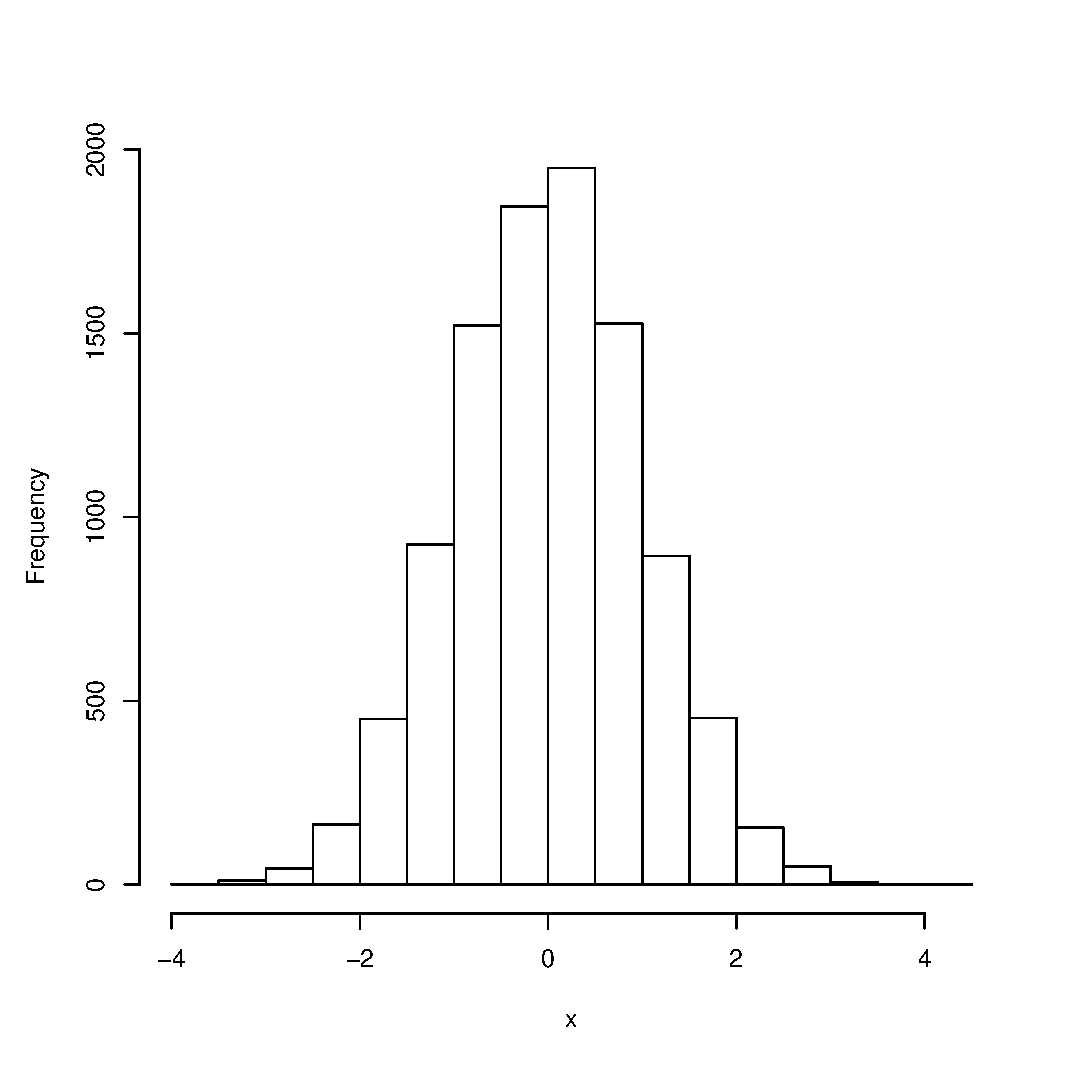
\includegraphics[width=10cm]{figures/StoreResultsHistRand10000Z-1} 
\SVGLink{StoreResultsHistRand10000Z-1} 
\end{center} 
\end{exhibit} 

 
It should be fairly obvious what each command does so the only one that really needs further explanation is the \Rcmd{savePlot} command. The first argument is the intended filename for our graph. The filename may need some further explanation. It is in several parts --- \code{$.\backslash\backslash$figures$\backslash\backslash$HistRandValsStandNorm.eps} has a path, a filename and the extension. 
 
The \code{$.\backslash\backslash$figures$\backslash\backslash$} is the path that shows \R{} to save the file in a subfolder off the current working directory. I've called the file \code{HistRandValsStandNorm.eps} because I want to use \LaTeX{} to compile these notes into a presentable document. 
Note that I have explicitly stated the extension in the complete filename to be the same as the second argument for the entire command, ``eps" in this instance. You can change this to suit other file types that you might need using \code{find/replace} techniques in your script files. Other file types available include ``jpg", ``bmp", and ``pdf". See the help on the \Rcmd{savePlot} command for a complete listing. 
 
The \Rcmd{x11} command can be replaced by a number of others which are all aliased with one another. The example above doesn't supply any arguments to this command, but width and height quantities can be supplied. The default size is 7$\times$7 inches but apparently this doesn't always behave properly under the Windows operating system. You might be advised to re-run the code above with the first command replaced by \code{x11(7,5)} or similar, changing the second number to alter the aspect ratio of the resulting figure window. Once you get the size you want for certain types of graphs you're bound to look back to your old code and replicate the same size graph windows every time. A boxplot is a key example where the default window size is often inappropriate. 
 
\section{Saving output in a text file}\label{TextSink} 
 
One simple way to redirect the output from the main \R{} window is to use the \Rcmd{sink} command. In this case, you will type in or execute commands as per normal but not see any of the output as this is appended to a separate text file. Try the following code on for size. 
 
\begin{Schunk}
\begin{Sinput}
> x=1:20 
> x 
\end{Sinput}
\begin{Soutput}
 [1]  1  2  3  4  5  6  7  8  9 10 11 12 13 14 15 16 17 18
[19] 19 20
\end{Soutput}
\end{Schunk}
\begin{Schunk}
\begin{Sinput}
> sink(".\\other\\JustPrintX.txt")
> x
> ## sink()
\end{Sinput}
\end{Schunk}
 
This creates a text file called \file{JustPrintX.txt} in a subfolder called \file{other}, within the current working directory (which I created earlier). The file is worth looking at because it should show exactly what would have been printed in the \R{} window if the sink were not active. Note that the second use of \code{sink()} stops the sink from being active. 
 
Just typing the name of an object implicitly calls the relevant \Rcmd{print} function for that object type. This does not work when a sink is active however, so we must use the \Rcmd{print} command explicitly to get the output into our sink file. For example 
\begin{Schunk}
\begin{Sinput}
> sink(".\\other\\JustPrintX2.txt")
> print(x)
\end{Sinput}
\begin{Soutput}
 [1]  1  2  3  4  5  6  7  8  9 10 11 12 13 14 15 16 17 18
[19] 19 20
\end{Soutput}
\begin{Sinput}
> ## sink()
\end{Sinput}
\end{Schunk}
Check this file out and note the contents are what we might expect. It's cleaner to use the \Rcmd{cat} command in place of the \Rcmd{print} command here though. For example 
\begin{Schunk}
\begin{Sinput}
> sink(".\\other\\JustPrintX3.txt")
> cat(x)
\end{Sinput}
\begin{Soutput}
1 2 3 4 5 6 7 8 9 10 11 12 13 14 15 16 17 18 19 20
\end{Soutput}
\begin{Sinput}
> ## sink()
\end{Sinput}
\end{Schunk}
An even quicker method useful for a single result is to use the \Rcmd{cat} command's full potential: 
\begin{Schunk}
\begin{Sinput}
> cat(x, file=".\\other\\JustCatX.txt") 
\end{Sinput}
\end{Schunk}
 
 
\section{Saving the entire \R{} Console} 
 
Windows users of \R{} who use the RConsole have an option to save the entire console using the menus. At present, however, this is not an option that can be invoked via the command line. 
 
It is possible to save the history of commands using the \Rcmd{savehistory} command, and of course your data and command history can be saved at the end of a session. 
 
You'll soon see that you do not need to save a copy of the \R{} console as it takes so little time to re-run a set of commands and re-generate the output desired. 
 
 
 

